\section{Setting The Tempo Of The Project}
\begin{itemize}
    \item First create a set by going to File $>$ New Live Set.
    \item The tempo is the speed or the beats per minute, depending on the song you are composing the tempo will be different.
        \begin{figure}[H]
            \centering
            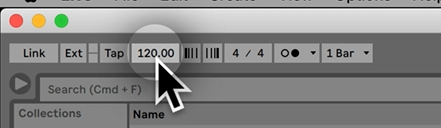
\includegraphics[width=\width\textwidth]{./figs/20220603195452.png}
            \caption{Tempo}
        \end{figure}

    \item By pressing the space bar you can hear the metronome at the beats per minute specified.
        \begin{figure}[H]
            \centering
            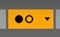
\includegraphics[width=\width\textwidth]{./figs/20220603195540.png}
            \caption{Metronome}
        \end{figure}
    
    \item The tap button can be used to adjust the beats per minute of your project. Every time you tap, ableton will adjust the beats per minute.
        \begin{figure}[H]
            \centering
            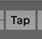
\includegraphics[width=\width\textwidth]{./figs/20220603195654.png}
            \caption{Tap button}
        \end{figure}
\end{itemize}

%%%%%%%%%%%%%%%%%%%%%%%%%%%%%%%%%%%%%%%%%%%%%%%%%%%%%%
\section{Audio tracks}
\begin{itemize}
    \item In session view we had the columns the capacity to hold you midi and audio tracks. We already saw sort of what is midi, the audio tracks we left pending.
        \begin{figure}[H]
            \centering
            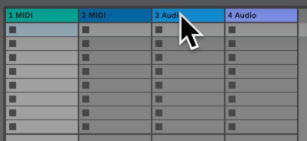
\includegraphics[width=\width\textwidth]{./figs/20220603200049.png}
            \caption{}
        \end{figure}
    \item Audio tracks hold audio files, these can be prerecorded sounds, or tracks, or even recodings.
    \item With audio tracks you don't need to load an instrument.
    \item You can add an audio track by selecting a track from the samples tab in Categories.
    \item Once you choose the track you like you can just drag and drop it to an audio slot. If you double click the track it will open the sample display in the clip view which will represent the wave form graph.
        \begin{figure}[H]
            \centering
            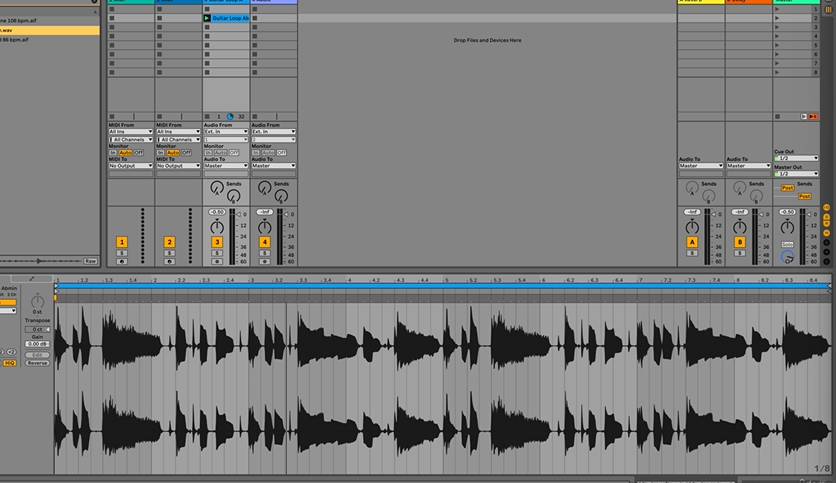
\includegraphics[width=\width\textwidth]{./figs/20220603200302.png}
            \caption{}
        \end{figure}
    
    \item You can move the clips by selecting them and droping in them in another slot and you can delete them by selecting them and pressing delete in your keyboard.
\end{itemize}

%%%%%%%%%%%%%%%%%%%%%%%%%%%%%%%%%%%%%%%%%%%%%%%%%%%%%%
\section{MIDI tracks}
\begin{itemize}
    \item MIDI tracks allow you to create music using virtual instruments. You can edit midi tracks and once you are done it can be played by a virtual instrument. Audio tracks are pre-recorded and you cannot easily change it, midi tracks are editable and you can actually draw in notes:
        \begin{figure}[H]
            \centering
            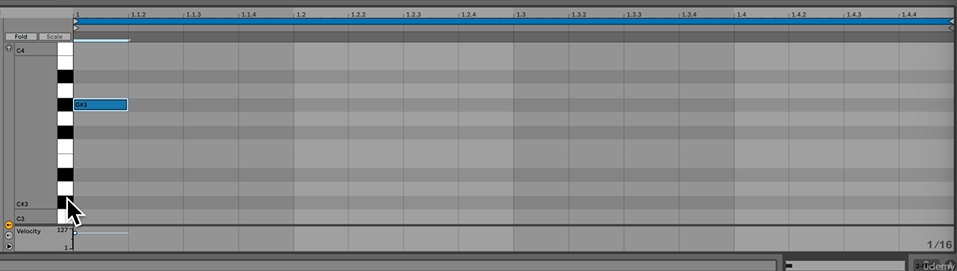
\includegraphics[width=\width\textwidth]{./figs/20220603201031.png}
            \caption{MIDI}
        \end{figure}
    
    \item You can draw a note by double clicking and you can change the length of it by selecting it and making it longer.
        \begin{figure}[H]
            \centering
            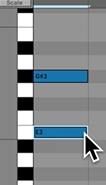
\includegraphics[width=\width\textwidth]{./figs/20220603201123.png}
            \caption{Creating a MIDI note}
        \end{figure}
    
    \item If you play midi and it doesn't sound, it is simply because you have not selected a virtual instrument. Select one and the drawed notes will sound. You can select an instrument in the Categories $>$ Intruments $>$ Your instrument. Then drag and drop your chosen instrument into the midi column.
\end{itemize}

%%%%%%%%%%%%%%%%%%%%%%%%%%%%%%%%%%%%%%%%%%%%%%%%%%%%%%
\section{Computer MIDI keyboard}
\begin{itemize}
    \item You can use your QWERTY keyboard to make sound too, drawing the notes with your mouse can get tedious, you can activate computer keyboard midi by clicking a button in the upper right corner that looks like this:
        \begin{figure}[H]
            \centering
            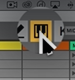
\includegraphics[width=\width\textwidth]{./figs/20220603201734.png}
            \caption{Computer midi keyboard}
        \end{figure}
    
    \item Then you need to select the midi column that will recieve the information, tell ableton which midi track will be the one that recieves the keyboard presses by clicking this button:
        \begin{figure}[H]
            \centering
            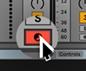
\includegraphics[width=\width\textwidth]{./figs/20220603201841.png}
            \caption{}
        \end{figure}
    
    \item The computer will map the computer's keyboard to a musical note:
        \begin{figure}[H]
            \centering
            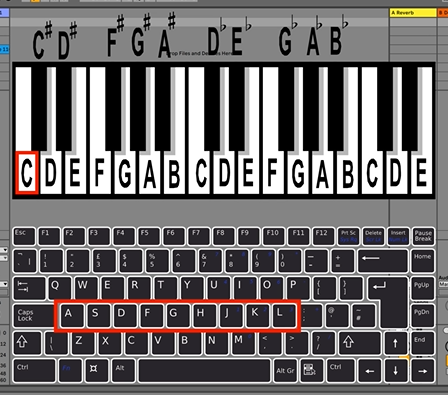
\includegraphics[width=\width\textwidth]{./figs/20220603201942.png}
            \caption{}
        \end{figure}
    
    \item The Z and X keys are used to augment or decrement the notes by one octave. Pressing Z will make all the notes an octave lower, pressing X will make all the notes an octave higher.
        \begin{figure}[H]
            \centering
            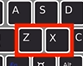
\includegraphics[width=\width\textwidth]{./figs/20220603203032.png}
            \caption{}
        \end{figure}
    
    \item By pressing M you can turn the computer midi keyboard on or off.
\end{itemize}

%%%%%%%%%%%%%%%%%%%%%%%%%%%%%%%%%%%%%%%%%%%%%%%%%%%%%%
\section{Setting up a MIDI controler}
\begin{itemize}
    \item A midi controler is a device that let's you to transmit midi notes or midi data using buttons or keys. 
    \item Midi devies must be set up correctly in ableton live.
\end{itemize}